\documentclass{article}

%install your packages here 
\usepackage[utf8]{inputenc}
\usepackage{amssymb}
\usepackage{amsmath}
\usepackage{mathtools}
\usepackage{amsthm}
\usepackage{setspace}
\usepackage{cancel}
\usepackage{bbm}
\usepackage{pgfplots}
\usepackage{listings}
\usepackage{multicol}
\usepackage{diagbox}
\usepackage{ tipa }
\usepackage{hyperref}
\usepackage{float}
\hypersetup{
    colorlinks=true,
    citecolor=black,
    filecolor=black,
    linkcolor=black,
    urlcolor=black
}

\usetikzlibrary{arrows, calc, patterns, shapes}
  \pgfplotsset{compat=1.15}
\renewcommand{\baselinestretch}{1.25}
\newcommand\sbullet[1][.5]{\mathbin{\vcenter{\hbox{\scalebox{#1}{$\bullet$}}}}}

%theorems
\theoremstyle{definition}
\newtheorem{theorem}{Theorem}

\theoremstyle{definition}
\newtheorem{definition}{Definition}

\newtheorem{example}{Example}[section]

%write short hand notes here 
%standard stats
\def\E{\mathbb{E}}
\def\l{\ell}
\def\xs{\{x_1, \hdots, x_n\}}
\def\Xs{\{X_1, \hdots, X_n\}}

%standard cal
\def\j{\mathcal{J}}
\def\sumn{\sum^n_{i=1}}
\def\inv{^{-1}}
\def\w{\omega}
\def\R{\mathbb{R}}
\def\fish{\mathcal{I}}
\def\v{\vec{v}}
\def\V{\Vec{V}}
\def\f{\mathcal{F}}

%symbols
\newcommand{\dotrel}[1]{\mathrel{\dot{#1}}}



\title{Math 806222 - Analysis of Extreme Values}
\author{Jean }
\date{Fall 2020}

\begin{document}
%makes the title and initial page
\maketitle
\tableofcontents{}
\pagebreak

\section{Introduction}
\subsection{Motivation}
This class has for focus the analysis of extreme values. This is not to be confused with extreme value theory. Theorems, lemmas, and concepts in this course will be defined and applied but not necessarily fleshed out or proved. These details can be found in the supplementary suggested readings. The tools from this class can be applied to finance, economics and financial engineering.
\subsection{Modeling}
\begin{definition}[Statistical Modeling] The use of sample data to make inferences of the probability structure of the population from which the data arose is referred to as \textbf{statistical modeling}.
\end{definition}
Given $\xs$ as independent (but not necessarily identically distributed) realisations/observations from a population of interest, in order to make any inference on these observations, we must first estimate the distribution. There are two methods for distribution estimation: \textbf{parametric modeling}, and \textbf{non-parametric modeling}. As we will see, the parametric approach is more suitable for extreme value analyses while the non-parametric method is only useful to capture some dependency issues.

\section{Parametric Modeling}
There are three steps to parametric modeling:
\begin{enumerate}
    \item Choosing a family of models within which the distribution of the data is assumed to lie
    \item Finding the family member from (1) that best corresponds to the data at hand
    \begin{enumerate}
        \item Parameter estimation
        \item Confidence interval for estimates
    \end{enumerate}
    \item Model diagnostics and evaluation
\end{enumerate}

\subsection{Choosing a Family}
Once we choose a family, we assume, for the rest of our parametric modeling, that the chose family was correct. It is important to note that once we have chosen, there is no way to correct for having chosen the wrong family. The choice of family is made based on:
\begin{itemize}
    \item \textbf{Physical Grounds:} what the process that sourced our data actually entails. (i.e. if we were observing coin flips we would use Binomial, if we were observing counts we would use Poisson).
    \item \textbf{Empirical Grounds:} what the exploratory analysis shows (i.e. if $\bar{x}\approx s$ then we might want to use an exponential family).
    \item \textbf{Limit Laws:} using an approximate model (i.e. Central Limit Theorem)
\end{itemize}

\subsection{Parameter Estimation}
Let $\xs$ be independent observations of random variables with a probability density function that is in a known familly of functions:
\[\mathcal{F} = \{f(x,\theta); \theta\in\Theta \} \]
with $\theta$ as either a scalar or a $d$-dimensional vector. Let $\theta_0$ be the true value of $\theta$ that generated our observed data. To estimate this unknown parameter, we can use any of the following:
\begin{itemize}
    \item Maximum likelihood estimation
    \item Method of moments
    \item Probability weighted methods
    \item Bayesian methods
    \item Robust methods of estimation
\end{itemize}

\subsubsection{Brief Review of Maximum Likelihood Estimation}
\begin{definition}[Likelihood Function] The probability of the observed data as a function of an unknown parameter $\theta$ is called the \textbf{likelihood function}. Assuming the observations are independent, the likelihood function is
\[\mathcal{L}(\theta)=\prod_{i=1}^n f_i(x_i; \theta)\]
with $f_i$ being the pdf/pmf of the i$^{th}$ observation. In practice, since the $\log$ function is monotonically increasing, maximizing the likelihood is equivalent to maximizing the log-likelihood. So we instead maximize 
\[\l(\theta)= \log(\mathcal{L}(\theta))= \sumn \log(f_i(x_i;\theta))\]

The maximum likelihood estimator $\hat{\theta}_0$ is defined by the value of $\theta$ that maximizes $\l(\theta)$. To get this, we must solve the equation below for $\theta$:
\[\frac{\partial}{\partial \theta} \l(\theta)=0\]
which can be done by hand or using the \texttt{optim} function from \texttt{R}.
\end{definition}

\subsection{Confidence Intervals}
Once we have estimated our parameter $\theta$, we need to build confidence intervals for the true parameter in order to evaluate the accuracy of our estimate.

\begin{definition}[Expected Information Matrix] The \textbf{expected information matrix}, also known as the \textbf{Fisher information matrix} measures the expected curvature of the log-likelihood and has information about the variability of estimated parameters. Assuming $\theta$ is $d$-dimensional, the EIM is represented by 
\[\fish_E(\theta)= \begin{bmatrix}e_{11}(\theta) &\hdots &\hdots & e_{1d}(\theta)\\
\vdots& \ddots & & \vdots\\
\vdots& &\ddots & \vdots\\
e_{d1}(\theta)& \hdots & \hdots& e_{dd}(\theta)\\
\end{bmatrix}\]
Where 
\[e_{ij}(\theta)=\E\bigg\{- \frac{\partial^2}{\partial \theta_i\partial\theta_j}\l(\theta) \bigg\}\]
\end{definition}


\begin{definition}[Observed Information Matrix]
This is an approximation of the expected information matrix. Since $\theta$ is rarely known, in practice, we use the \textbf{observed information matrix}:
\[\fish_O(\theta)= 
\begin{bmatrix}-\frac{\partial^2}{\partial \theta_1^2}\l(\theta)  &\hdots &\hdots & -\frac{\partial^2}{\partial \theta_1\partial\theta_d}\l(\theta) \\
\vdots& \ddots & & \vdots\\
\vdots& &\ddots &\vdots \\
-\frac{\partial^2}{\partial \theta_d\partial\theta_1}\l(\theta) & \hdots & \hdots& -\frac{\partial^2}{\partial \theta_d^2}\l(\theta) \\
\end{bmatrix}\]
This can be manually calculated or retrieved from the \texttt{optim} function in \texttt{R}.
\end{definition}

\begin{theorem}
Under suitable regularity conditions, for large $n$, 
\[\hat{\theta}_0 \dotrel{\sim} \textit{MVN}\Big(\theta_0, \fish_{E}(\theta_0)\inv \Big)\]
Where $\dotrel{\sim}$ means ``approximately distributed as". If $\theta$ is multidimensional, we can break this down. First, we denote $\fish_{E}(\theta_0)\inv$ as $\Psi_{i,j}$. Then, for all $\theta_i$ in $\theta_0=(\theta_1,\hdots, \theta_d)$, we have 
\[\hat\theta_i\dotrel{\sim} N(\theta_i, \Psi_{ii})\]
This can be used to build confidence intervals for $\theta_i$. Note that in practice, $\fish_O(\hat{\theta})$ is used instead of $\fish_E(\theta_0)$.

This theorem holds when we have many observations (large $n$). In many (most) extreme values problems, by the very nature of extreme value statistics, we simply do not have enough samples to apply Theorem 1. Additionally, for some extreme value problems, the regularity conditions that Theorem 1 assumes are not satisfied.
\end{theorem}
\begin{theorem}
Let $\phi=g(\theta)$ where $g$ is a scalar function. If $\hat{\theta}_0$ is the maximum likelihood estimator (MLE) for $\theta_0$, then, the MLE for $\phi$ is $\hat{\phi}_0=g(\hat{\theta}_0)$
\end{theorem}

\begin{theorem}As above, let $\phi=g(\theta)$. Furthermore, let $\hat{\theta}_0$ be the large sample MLE of the $d$-dimensional parameter $\theta_0$ with approximate variance-covariance matrix $V_{\theta}$. Then, it follows that

\[\hat{\phi}_0\dotrel{\sim} N(\phi_0, V_\phi)\]
where 
\[V_\phi= \nabla \phi^T V_\theta\nabla \phi\]
and
\[\nabla\phi=\bigg[ \frac{\partial \phi}{\partial\theta_1}, \hdots,\frac{\partial \phi}{\partial\theta_d} \bigg] \hspace{.3cm} \text{evaluated at }\hat{\theta}_0\]
computing an estimate of the variance of $\hat{\phi}_0$ using $V_{\theta}$ is known as the \textbf{delta method}
\end{theorem}
\subsubsection{Deviance}
Another method of creating confidence intervals is through the use of the \textbf{deviance function}:
\[D(\theta)= 2\{ \underbrace{\l(\hat{\theta}_0)}_{\text{largest likelihood}} - \underbrace{\l(\theta)}_{\text{likelihood at some other $\theta$}}\}\]
Once we have the deviance function, a natural criterion for a confidence region using a threshold $c$ is to define the region as
\[CR=\{\theta| D(\theta)\leq c\}\]

\begin{theorem}For large $n$, under suitable regularity conditions, 
\[D(\theta_0)\dotrel{\sim} \chi^2_d\]
From this theorem, it follows that a $(1-\alpha)100\%$ confidence interval for $\theta_0$ is given as 
\[C_\alpha= \{\theta| D(\theta)\leq \chi_{\alpha,d}^2\}\]
where is the upper $\alpha$-quantile of a $\chi^2$ distribution with $d$ degrees of freedom. This method of creating confidence intervals is usually more accurate then Theorem 1.
\end{theorem}
Since bounds from Theorem 4 often outperform those from Theorem 1, it is of interest to see if we can apply a similar method to get confidence intervals for individual $\theta_i$. To do this, we will need one more tool.
\begin{definition}[Profile Likelihood]
Let $\theta_{-i}$ denote all the vector components of $\theta$ except $\theta_i$. Then, the \textbf{profile likelihood}(PLL) for $\theta_i$ is defined as 
\[\l_p(\theta_i)= \max_{\theta_{-i}}\l(\theta_i, \theta_{-i})\]
This means that for each value $\theta_i$, the PLL is the maximized log likelihood over all other ($d-1$) components of $\theta$.
\end{definition}

\begin{theorem}For large $n$, under suitable regularity conditions, we can recover the \textbf{profile deviance}:
\[D_p(\theta_i)= 2 \{ \l(\hat{\theta}_0) - \l_p(\theta_i)\}\dotrel{\sim} \chi^2_1\]
From this, it follows that a $(1-\alpha)100\%$ confidence interval for $\theta_i$ is
\[C_\alpha = \{\theta_i | D_p(\theta_i)\leq \chi^2_{\alpha,1}\}\]
where $\theta_i$ in $C_\alpha$ represents possible values of the $i^{th}$ component of $\theta$ rather than the true value of the $i^{th}$ component.
Now, let us examine the retaining criterion in the RHS of the equation above:
\begin{align*}
    &D_p(\theta_i)\leq \chi_{\alpha,1}^2\\
    &=2 \{ \l(\hat{\theta}_0) - \l_p(\theta_i)\} \leq \chi_{\alpha,1}^2\\
    &= \l(\hat{\theta}_0) - \l_p(\theta_i) \leq \frac{\chi_{\alpha,1}^2}{2}\\
    &= \l_p(\theta_i) \geq \l(\hat{\theta}_0) -\frac{\chi_{\alpha,1}^2}{2} \tag{*}
\end{align*}
In practice, we build the the PLL function $\l_p(\theta_i)$ and find the range of values $\theta_i$ such that (*) holds.
\end{theorem}

\begin{definition}[Deviance Statistic]
Theorem 5 can be used for model selection. Let $M_1$ be a model with parameter $\theta$, $M_0$ be a subset of $M_1$ where $k$ of the components of $\theta$ are constrained to 0, and let $\l_j(M_j)$ be the corresponding log-likelihood for model $j$. The \textbf{deviance statistic} is
\[D=2\{\l(M_1) - \l(M_0)\}\]
\end{definition}

\begin{theorem}Let
\begin{align*}
    \mathcal{H}_0: & M_0 \text{ is valid}\\
    \mathcal{H}_A: & M_1 \text{ is a better fit}
\end{align*}
We reject $\mathcal{H}_0$ in favor of $\mathcal{H}_A$ if 
\[D=2\{\l(M_1) - \l(M_0)\}>\chi^2_{\alpha,k}\]
\end{theorem}
\subsection{Model diagnostics}
Remember, nowhere in our parametric modeling have we accounted for choosing the wrong family. Here, we assess how well the model we assumed fits to the data we have. Ideally, we would use cross validation on one or more held out sets. However, since we are dealing with extreme value statistics, we will rarely have enough data to use this method. In practice, we instead evaluate the concordance between our model and the data it estimates.
\begin{definition}[Empirical Distribution Function]
Given an ordered sample of independent observations:
\[x_{(1)}\leq \hdots \leq x_{(n)} \]
from a population with \textbf{true} cumulative distribution function $F$, we define the \textbf{empirical distribution function} as

\[\Tilde{F}(x)=\frac{i}{n+1} \hspace{1cm} \text{for } x_{(i)}\leq x< x_{(i+1)}\]
\end{definition}
Let $\hat{F}$ be an estimate for $F$ from our model. Then, it follows that $\Tilde{F}$ and $\hat{F}$ should be in agreement. In fact, there are various goodness of fit procedures based on comparisons of $\Tilde{F}$ and $\hat{F}$.

\begin{definition}[P-P plot] a \textbf{probability probability plot} (pp plot) consists of the points 
\[ \Bigg\{ \bigg(\hat{F}(x_{(i)}), \frac{i}{n+1}\bigg)| i=1, \hdots, n \Bigg\}\]
note that this is essentially the same as plotting our estimate of $\hat{F}$ from the model against the empirical distribution function $\Tilde{F}$. The goal here is to check that the empirical distribution function is aligned with the model estimate for the distribution function while accounting for the probability scale.
\end{definition}

\begin{definition}[Q-Q plot] a \textbf{quantile quantile plot} (qq plot) consists of the points 
\[ \Bigg\{ \bigg(\hat{F}\inv (\frac{i}{n+1}), x_{(i)}\bigg)| i=1, \hdots, n \Bigg\}\]

This plot is more focused on the comparing the tail behavior of $\hat{F}$ and $\Tilde{F}$. In a qq plot, we plot the quantiles of our model estimate against the quantiles of our empirical distribution function and hope they lign up.
\end{definition}
When running model diagnostics, it is important to use both a pp plot and a qq plot as they give the same information but on different scales.

\section{Fundementals of Extreme Value Theory}
Usually, we define $\Xs$ as our random values of interest measured on a time scale(i.e. daily stock, weekly rainfall, ...). These may or may not be iid observations but for now, let $\Xs$ be a sequence of iid observations with distribution function $F$. Consider the random variable
\[M_n=\max\Xs\]
In this section, we will focus on maxima but it is important to note that the same calculations can be done on minima (or simply changing the sign of observed values and sticking with max calculations). If $n$ is the number of observations in a year, then $M_n$ is the \textbf{annual maximum}. Furthermore, we can calculate its distribution
\[F_{M_n}(z)=P(M_n\leq z)= \prod_{i=1}^nF_{X_i}(z)=[F(z)]^n\]
If $F$ is known, then finding the distribution function of $M_n$ is fairly straightforward. In practice however, $F$ is not known. To find the distribution of $M_n$, we could try to find an estimate $\hat{F}$ and use it to calculate $\hat{M}_n\sim [\hat{F}]^n$ but we can see that small mistakes in the estimation of $F$ will grow into significant errors in the estimation of the distribution of $\hat{M}_n$ as $n \rightarrow \infty$. Instead, we look for approximating families to model $F^n$.

Let $z_+ $ the the smallest value such that $F(z)=1$. Then, for all $z<z_+$, we have 
\[\lim_{n\rightarrow \infty}F(z)^n=0\]
This means that the distribution of $M^n$ \textbf{degenerates} to a point mass at $z_+$ as $n\rightarrow \infty$ . To avoid dealing with such distributions, we allow for re-normalizations of $M_n$:
\[\frac{M_n- b_n}{a_n} \hspace{1cm} a_n>0\]
Where the right choice of sequences $a_n$ and $b_n$ stabilize the location and scale of $M_n$ as $n$ increases.

\subsection{Approximating Distributions for Maxima}
\begin{theorem}
Let $\w(F)=\sup\{x:F(x)<1\}=+\infty$\footnote{The cdf $F$ has a horizontal asymptote at y=1}. Furthermore, let us assume $\exists$ a constant $\alpha>0$ such that $\forall x>0$
\[ \lim_{t\rightarrow \infty} \frac{1-F(tx)}{1-F(t)}=x^{-\alpha} \tag{$\Delta$}\]
Here, $(\Delta)$ tells us how much probability there is in the tail and that $X$ is a \textbf{regularly varying} random variable. If the above holds, then $\exists$ a sequence $a_n>0$ such that 
\[\lim_{n \rightarrow \infty} P\bigg( \frac{M_n}{a_n} <x \bigg)= \begin{cases}\exp (x^{-\alpha}) & x>0\\
0 & x\leq 0
\end{cases}\]
and the sequence can be chosen as 
\[ a_n=\inf \bigg\{ x:1-F(x)\leq \frac{1}{n} \bigg\}\]
When this is the case, we say that F is in \textbf{the domain of attraction of Fréchet} and we write $F\in $MDA(Fréchet).
\end{theorem}

\begin{theorem}
Let $\w(F)$ be finite (i.e. if $F$ is uniform $\w(F)=1$). Furthermore. assume that the distribution function 
\[F^*(x)=F\bigg(\w(F)-\frac{1}{x}\bigg) \hspace{1cm} \forall x>0 \]
satisfies condition $(\Delta)$ from Theorem 7. Then, $\exists \{a_n\}, \{b_n\}$ such that 
\[\lim_{n\rightarrow \infty}P \bigg[ \frac{M_n-b_n}{a_n} < x\bigg]=\begin{cases}1 & x\geq 0\\
\exp(-x(-x)^\alpha)&x<0
\end{cases}\]
Where the normalizing constants can be chosen as 
\begin{align*}
    b_n&=\w(F)\\
    a_n&=\w(F)- \inf\{x:1-F(x)\leq \frac{1}{n}\}
\end{align*}
When this is the case, we say that F is in \textbf{the domain of attraction of Weibull} and we write $F\in $MDA(Weibull).
\end{theorem}

\begin{theorem}
Assume that for some finite $a$
\[\int_a^{\w(F)} (1-F(y))dy < \inf\]
Then, for $x$ in the range $\inf\{x:F(x)>0\}<x<\w(F)$, we define 
\[R(t)= (1-F(t))\inv \int_t^{\w(t)} (1-F(y))dy\]
Finally, assume that $\forall x \in \mathbb{R}$
\[\lim_{t\rightarrow \w(F)} \frac{1-F(t+xR(t))}{1-F(t)}\underset{\footnotemark}{=}e^{-x}\]
Then $\exists$ sequences $\{a_n\}>0,\{b_n\}$ such that 
\[\lim_{n\rightarrow \infty}P \bigg[ \frac{M_n-b_n}{a_n} < x\bigg]=\exp(-\exp(-x)) \hspace{0.5 cm} \forall x\in \mathbb{R}\]
Where the normalizing constants can be chosen as 
\begin{align*}
    b_n&=\inf\{x:1-F(x)\leq \frac{1}{n}\}\\
    a_n&=R(b_n)
\end{align*}
When this is the case, we say that F is in \textbf{the domain of attraction of Gumbell} and we write $F\in $MDA(Gumbell).
\footnotetext{this means $F$ has (light) exponential tails. This forces a restriction on the decay of the distribution}

\end{theorem}

Below are some notes on the last 3 theorems:
\begin{itemize}
    \item Theorems 7-9 exhaust all possibilities for the existence of the asymptotic distribution of maxima of iid rv (i.e. if F does not fall in any of the categories above then there are no normalizing constants that lead to a non-degenerate limit).
    \item The choice of constants $a_n,b_n$ is not unique. Changing these will yield a family with the same $\alpha$ parameter but (perhaps) different location and scale parameters
    \item In the past, we would choose one of the three proposed families to use to model $M_n$. Then, any inference made from this assumption would rely on the presupposition that we had made the correct choice of family. Now of course, there is a better solution.
\end{itemize}

\subsection{Generalized Extreme Value Family}
\begin{theorem}
If there exists sequences $\{a_n\},\{b_n\}$ such that 
\[\lim_{n\rightarrow\infty}P \bigg[\frac{M_n-b_n}{a_n}\leq z \bigg]=G(z)\tag{$\diamond$}\]
for a non-degenerate distribution function $G$, then $G$ is a member of the \textbf{generalized extreme value }(GEV) family and can be written as 
\[G(z)=\exp\bigg\{ - \bigg[1+\xi \bigg(\frac{z-\mu}{\sigma}\bigg)\bigg]^{-\frac{1}{\xi}}\bigg\}\]
defined on 
\[\{z:\bigg[1+\xi \bigg(\frac{z-\mu}{\sigma}\bigg)\bigg]^{-\frac{1}{\xi}}>0\}\]
Below are the parameter specifications of a GEV distribution.
\begin{itemize}
\item $\mu\in\R $ is a location parameter
\item $\sigma\in\R^+$ is a scale parameter
    \item $\xi\in \R$ is a shape parameter
\end{itemize}
\end{theorem}
\subsection{Properties of GEVs}
\subsubsection{Statistical properties}
Let $X\sim GEV(\mu, \sigma,\xi)$, then
\begin{align*}
    \E(X)&=\mu+\frac{\sigma}{\xi}(g_1-1)\\
    Var(X)&=\frac{\sigma^2}{\xi^2}(g_2-g_1^2)\\
    Mode(X)&=\mu+\frac{\sigma}{\xi}[(1+\xi)^{-\xi} -1]
\end{align*}
Where \[g_k=\Gamma(1-k\xi)\hspace{1cm} k\in\{1,2\}\]
and 
\[\Gamma(x)=\int_0^{\infty}t^{x-1}e^{-t}dt\]
\subsubsection{Analytic Properties}
Since a $GEV$ is defined on $1+\xi \bigg(\frac{z-\mu}{\sigma}\bigg)>0$, it follows that there is an upper bound on $x$ when $\xi<0$ and a lower bound when $\xi>0$
\[\begin{cases}
x < \mu-\frac{\sigma}{\xi}& \text{if }\xi<0\\
x > \mu-\frac{\sigma}{\xi}& \text{if }\xi>0
\end{cases}\]
Furthermore, assuming $(\diamond)$ holds for large enough values of $n$, we have 
\begin{align*}
    G(z)&\approx P \bigg[\frac{M_n-b_n}{a_n}\leq z \bigg]\\
    \implies P(M_n\leq z)& \approx G\bigg(\frac{z-b_n}{a_n}\bigg)\\
    &=G^*(z)
\end{align*}
Where $G^*$ is another member of the $GEV$ family.
\begin{definition}[Max-stability] A distribution is said to be \textbf{max-stable} if $\forall n=\{2,3,\hdots\}$, there are constraints $\alpha_n,\beta_n$ such that 
\[G^n(\alpha_nz+\beta_n)=G(z)\]
Where $G^n$ is the distribution of $M_n$. This definition shows that max-stable distributions are those where the sample maxima leads to identical distribution apart from a change of scale and location. 

\end{definition}
\begin{theorem}
A distribution is max-stable iff it is a GEV.
\end{theorem}
\noindent With this result, we can derive the following ``proof'' for Theorem 10. First, we know that for large enough $n$,
\[P\bigg[\frac{M_n-b_n}{a_n}\leq z \bigg]  \approx G(z)\]
Then, for any integer $k$, $nk$ is at least as large as $n$ so
\[P\bigg[\frac{M_{nk}-b_{nk}}{a_{nk}}\leq z \bigg]  \approx G(z) \tag{$\clubsuit$}\]
But since $M_nk$ is the maximum of $k$ variables having the same distribution as $M_n$, we have
\[P\bigg[\frac{M_{nk}-b_{nk}}{a_{nk}}\leq z \bigg] =\bigg( P\bigg[\frac{M_n-b_n}{a_n}\leq z \bigg]\bigg)^k \tag{$\spadesuit$}\]
So we have
\begin{align*}
    (\clubsuit)&\implies P(M_{nk}\leq z)\approx G(\frac{z-b_{nk}}{a_{nk}})\\
    (\spadesuit)&\implies P(M_{n}\leq z)\approx G^k(\frac{z-b_n}{a_n})
\end{align*}
Which shows that $G$ is max-stable and therefore, a $GEV$.


\section{Modeling Univariate Extremes}
\subsection{Block Maxima}
Given independent observations of $\{x_1,x_2,\hdots\}$, of data block (or separate) into sequences of observations each having length $n$ for large $n$. This generates the sequence of maxima $\{M_{n,1},\hdots,M_{n,m}\}$ to which we can fit a $GEV$. See now we split our data into maximal data and use the distribution of max-like data for interpretation. Note: the choice of block size is critical. It gives rise to the standard bias-variance trade-off we often come across in statistics. Having blocks that are too small may mean that the approximation by the limit model is likely to be poor whereas having large blocks generate few block maxima, thus leading to a large estimation variance. For this section, let us consider the maximum likelihood estimator for GEVs.

Since the support of a GEV depends on the parameters, we see that it is possible to run into difficulties when making the regularity assumptions that so many of our MLE theorems depend on. For this reason, we analyse 3 cases:
\begin{enumerate}
    \item $\xi>-0.5$: This yields a \textbf{regular} MLE and we can make the standard normality assumptions
    \item $-1<\xi<-0.5$: We can usually optain an MLE but these do not have the standard asymptotic properties
    \item $\xi<-1$: MLE are likely to be unobtainable.
\end{enumerate}

Let $\{z_1,\hdots,z_m\}$ denote the block maxima assumed to be independent random variables following a GEV distribution; the MLE can be found through likelihood function:
\[\l(\mu,\sigma,\xi)=-m\log(\sigma)-(1+\frac{1}{\xi})\sum_{i=1}^m \log[1+\xi(\frac{z_i-\mu}{\sigma})]- \sum_{i=1}^m[1+\xi(\frac{z_i-\mu}{\sigma})]^{-1/\xi}\]
provided of course that \[1+\xi(\frac{z_i-\mu}{\sigma})>0\hspace{1cm}  i=1,2,\hdots,m\]
Otherwise, the likelihood is 0 and the log-likelihood is $-\infty$ for that observation. It is important to note that there is no analytical solution for the MLE of a GEV. Numerical approximations must be used 
on a re-parameterized log-likelihood to obtain the best estimates.

\subsubsection{Quantiles}
When analyzing extreme data, the quantities of interest are usually the extreme upper quantiles of the (annual) maximum distribution. To do this, we invert $G(z_p)=1-p$ to find
\[z_p=\begin{cases} \mu-\frac{\sigma}{\xi}[1-\{-\log(1-p)\}^{-\xi}] & \xi\neq 0\\
\mu-\sigma\log\{-\log(1-p)\}&\xi= 0
\end{cases} \tag{**}\]
We refer to the \textbf{return level} $z_p$ associated with the \textbf{return period} $\frac{1}{p}$. For example, if we were observing annual rain data, $z_p$ would be the amount of rain  expected to be exceeded on average once every  $\frac{1}{p}$ years. Or $z_p$ is expected to be exceeded by the annual maximum once ever  $\frac{1}{p}$ years.

We can let $y_p=-\log(1-p)$ and plot $z_p$ from $(**)$ against $y_p$ on a log scale. When we do this we observe 3 distinct behaviors:
\begin{enumerate}
    \item $\xi=0$: the plot is linear
    \item $\xi>0$: the plot is convex with no finite bound
    \item $\xi<0$: the plot is concave with an asymptotic limit as $p\rightarrow 0$
\end{enumerate}
In practice, we want to estimate $z_p$. To do so using normality, we substitute the MLE into $(**)$ and use the delta method to obtain a 95\% confidence interval. This yields mixed results as the normal approximation for the MLE may be poor (especially $\hat{\xi},\hat{z}_p $)
\subsubsection{Profile Likelihood}
Instead of the delta method, we can use the profile likelihood to create our confidence interval for $Z_p$ using Theorem 4. We first, reparameterize the likelihood function using
\[\mu=z_p+\frac{\sigma}{\xi}[1-\{-\log(1-p)\}^{-\xi}]\]
Then, we consider the likelihood function as a function of $z_p$:
\[l(z_p)= \max_{\xi, \sigma}\l(z_p,\xi, \sigma)\]

\subsection{$r$ Largest Statistics}
The next approach to building models for univariate extremes focuses on applying what we have learned from the block maxima approach to more observations of data. Let $\Xs$ be a sequence of iid random variables. Furthermore, let $M_n^{(k)}$ be the $k^{th}$ largest observation from said sequence.
\begin{theorem}
If there exist sequences $\{a_n\}, \{b_n\}$ such that 
\[\lim_{n\rightarrow \infty} P \bigg[ \frac{M_n-b_n}{a_n}\leq z \bigg]= G(z)\]
For some non degenerate distribution function $G$\footnote{By theorem 10, $G$ is a GEV}. Then, for a fixed value $k$,
\[\lim_{n\rightarrow \infty} P \bigg[ \frac{M_n^{(k)}-b_n}{a_n}\leq z \bigg]= G_k(z)\]
on $\{z:1+\xi(z-\mu)/\sigma > 0\}$, where

\[G_k(z)=\exp\{-\tau(z)\}\sum_{s=0}^{k-1}\frac{\tau(z)^s}{s!} \hspace{1cm} \text{with }\tau(z)=\bigg[1+\xi\bigg(\frac{z-\mu}{\sigma}\bigg)\bigg]^{\frac{-1}{\xi}} \]
We note that $M_n^{(k)}$ must be normalized in the same fashion as $M_n$, and shares the same GEV parameters. To model a single maximum, we can use $G_k(z)$.
\end{theorem}
A more interesting application of this theorem, would be to use it to augment the number of observations in our block maxima technique. Consider the vector quantity
\[\tilde{M}_n^{(r)} = (M_n^{(1)},\hdots, M_n^{(r)})\]
From the theorem above, we can get the approximate distribution of each of its sub components and evaluate this fit using qq and pp plots. However, we are more interested in their joint distribution $\tilde{M}_n^{(r)}$. Clearly, we cannot use the i.i.d. assumption, as the components are not independent.
\begin{theorem}
If there exist sequences $\{a_n\},\{b_n\}$ such that 
\[\lim_{n\rightarrow \infty} P \bigg[ \frac{M_n-b_n}{a_n}\leq z \bigg]= G(z)\]
For some non degenerate distribution function $G$, then, for a fixed $r$ the limiting distribution as $n \rightarrow \infty$ of
\[\tilde{M}_n^{(r)}= \bigg(\frac{M_n^{(1)}-b_n}{a_n},\hdots, \frac{M_n^{(r)}-b_n}{a_n} \bigg)\]
Falls within the families having joint distribution function 
\[f(z^{(1)}, \hdots,z^{(r)})= \exp \bigg\{ -\bigg[ 1+ \xi \bigg( \frac{z^{(r)} -\mu }{\sigma}\bigg)\bigg]^{-1/\xi}\times \prod_{k=1}^r \sigma^{-1} \bigg[ 1+ \xi \bigg( \frac{z^{(k)} -\mu }{\sigma}\bigg)\bigg]^{-1/\xi-1}\bigg\} \]
With the $z^{(l}_s$ as ordered statistics. We must also ensure that $$\bigg[ 1+ \xi \bigg( \frac{z^{(k)} -\mu }{\sigma}\bigg)\bigg] >0 \hspace{1cm} \forall k=1,\hdots,r $$
\end{theorem}
This theorem gives use a method to fit r-largest statistics to data. In addition to still needing to define blocks and block sizes, we must also decide what values $r$ will take on. While large values of $r$ reduce the variance or our model estimators, these are more likely to violate the asymptotic conditions of the model (as $n\rightarrow \infty$ and $r$ is fixed). The larger our value for $r$, the larger $n$ must be before the conditions hold.
\subsection{Threshold Models}
Let $X_1, X_2, \hdots$ be a sequence of i.i.d random variables having a marginal distribution function $F$. In this method, we do not consider the maximum from each block but rather the exceedences over some high threshold $u$. From elementary application of Baye's rule, we note that 
\begin{align*}
    P(X>u+y|X>u)&=\frac{P[(X>u+y)\cap (X>u)]}{P(X>u)}\\
    &=\frac{1-F(u+y)}{1-F(u)} \hspace{1cm} y>0
\end{align*}
This probability can be seen as calculating the probability that we exceed threshold $u$ by $y$ given/knowing that we exceed threshold $u$. Of course, if $F$ is known, then so is the distribution of the threshold exceedences. As with $F^n$, we aim to have an asymptotic approximation for $P(X>u+y|X>u)$ as $u \rightarrow \infty$.
\begin{theorem}
Let $X_1,X_2,\hdots$ be a sequence of i.i.d. random variables with distribution function $F$ such that $F\in MDA(GEV(\mu,\sigma, \xi))$. Then, for large enough $u$,
\[F_u(y)= P(X-u>y|X>u)= 1-\bigg(1+\frac{\xi y}{\sigma^*} \bigg)^{-1/\xi}\]
where $y>0$, $1+\frac{\xi y}{\sigma^*} >0$, and $\sigma^*= \sigma+ \xi(u-\mu)$.
This limiting distribution corresponds to the generalized Pareto distribution. Below are the summary statistics for a $X\sim GP(\sigma, \xi)$ rv:
\begin{align*}
    \E(X)&=\frac{\sigma}{1-\xi} &\xi<1\\
    Var(X)&= \frac{\sigma^2}{(1-\xi)^2(1-2\xi)}&\xi<1/2
\end{align*}
\end{theorem}
When $\xi>0$, then the $GP$ is defined on $[0,\infty)$; when $\xi<0$, then the $GP$ is defined on $[0,\frac{-\sigma}{\xi})$. Similarly to GEVs, the $\xi$ parameter in a GP is the denominating parameter. With $\xi<0$ the distribution of excess has an upper bound of $u- \tilde{\sigma}/\xi$. Inversely, with $\xi>0$ the distribution of excess has no upper limit. We interpret $\xi=0$ to be the limiting form of the distribution resulting in an exponential distribution:
\[H(y)= 1-\exp(-y/\tilde{\sigma})\]
Here are the steps to model extremes using threshold exceedences:
\begin{enumerate}
    \item Take the raw data $\xs$ and assume it to be i.i.d.
    \item Filter the data into exceedences over a threshold $\{x_i: x_i>u\}$
    \item Transform data points into the magnitude of the exceedences: $\{y_i =x_i-u\}$
    \item By theorem 14, these are approximately i.i.d. and form a GP distribution.
\end{enumerate}
One of the more important steps is figuring out the value of our threshold $u$. If we pick a low threshold, we risk violating the asymptotic basis for our model; if we pick too high a threshold, we will have few exceedences and therefore create a high variance model.
\subsubsection{Mean Residual Life Plots}
To find the ideal threshold(s), we use the \textbf{mean residual life} (MRL) plots. Suppose we are given an i.i.d. series $X_1, X_2, \hdots$. Then, if GP is a valid model with a threshold $u_0$, then, by theorem 14, it is also a valid model with threshold $u>u_0$. Now, we can calculate their expected value
\begin{align*}
    \E[X-u|X>u]&=\frac{\sigma_u}{1-\xi}\\&= \frac{\sigma_{u_0} +\xi(u-u_0)}{1-\xi}\\&= \frac{\sigma_{u_0} -\xi u_0}{1-\xi} + \frac{\xi}{1-\xi}u
\end{align*}
As we can see, the mean becomes a linear function of $u$ after we have crossed the minimal valid threshold. In an MRL plot, we plot $\frac{1}{n_u}\sum_{i=1}^{n_u}(x_i-u)$ vs $u$. Once the plot becomes a linear function of $u$, we can assume we have found the threshold. 

\subsubsection{Parameter Estimation}
Given a threshold $u$ and some data,  might wish to estimate $\sigma, \xi$. The log likelihood takes the form:
\[l(\sigma,\xi)= -k\log(\sigma) - \bigg( 1+\frac{1}{\xi}\bigg)\sum_{i=1}^k\log\bigg( 1+\frac{\xi y_i}{\sigma}\bigg)\]
However, it has no analytical solution and we must use numerical optimization algorithms to retrieve estimates. For $\xi=0$, we have 
\[\l(\sigma)= -k\log(\sigma)- \frac{1}{\sigma}\sum_{i=1}^ky_i\]
\subsubsection{Return Levels }
As with all of our extreme value models, it is often of interest to retrieve the return levels. Assuming $X\sim GP(\sigma,\xi)$
\begin{align*}
    P(X>x)&= P(X>x|X>u)P(X>u)\\
    &=\zeta_u \bigg[ 1+ \xi\frac{x-u}{\sigma} \bigg]^{-1/\xi}= \frac{1}{m}
\end{align*}
Where $P(X>u)=\zeta_u$. Solving the equation above to retrieve $m$ gives:
\[x_m= u+ \frac{\sigma}{\xi}[(m\zeta_u)^\xi -1]\]
Provided that n is large enough that $x_m>u$. If $\xi=0$, we have instead
\[x_m= u+\sigma\log(m\zeta_u)\]
As for before, we can plot $x_m$ vs $m$ on a logarithmic scale on observe the effects of $\xi$:
\begin{itemize}
    \item $\xi>0$ plot is convex
    \item $\xi=0$ plot is linear 
    \item $\xi<0$ plot is concave
\end{itemize}
We may also calculate the $N$ year return level. Given that there are $n_y$ observations per year, the $N$ year return level can be calculated as  
\[z_N= u +\frac{\sigma}{\xi}[(n_yN\zeta_u)^\xi -1]\]
To obtain estimates for $z_N$, we may simply use the sample parameter estimates $\hat{\sigma}, \hat{\xi}$ and $\hat{\zeta}_u= \frac{k}{n}$. Furthermore, as the number of exceedences is Binomial$(n, \zeta_u)$, we know $Var(\hat{\zeta}_u)= \frac{\hat{\zeta}_u(1-\hat{\zeta}_u)}{n}$, we can calculate a confidence interval for the $z_N$ using the delta method. Similar to what we observe with GEVs, confidence intervals for return levels from profile likelihood are more precise. From the likelihood function, we see that profiling for $\xi,\sigma$ is not difficult. Therefore, it is enough to write $\sigma$ as a function of either of these to profile $x_m$.
\[\sigma= \frac{(x_m-u)\xi}{(m\zeta_u)^\xi-1}\]
From here, we ignore the uncertainty due to $\zeta_u$ as it is usually small and instead focus on 
\[\max_{\xi}l(\xi, x_m)\]
To find our confidence interval for $x_m$


\section{Maxima For Stationary Sequences}
So far, we have assumed that we observe iid data. In reality, data rarely perfectly resembles iid sequences. For this reason, we must relax our constraint. We will generalize our approaches so far by seeing how they behave on data with different assumptions
\begin{definition}[Stationary Sequence] A sequence of random variables $(X_1,X_2, \hdots)$ is said to be \textbf{strictly stationary} if 
\[(X_{t_1},\hdots, X_{t_m}) \overset{d}{=} (X_{t_1+h},\hdots, X_{t_m+h}) \]
For any choice of indices $t_1<\hdots<t_m$, and integer $h$. 
\end{definition}
\begin{definition}[Second order stationary]
A strictly stationary sequence is said to be second order stationary if $\E[X_n]^2<\infty \forall n$, $\E[X_n]=\E[X] \forall n$, and $Cov(X_n, X_m)= Cov(X_0, X_{|m-n|})$
\end{definition}
Before we can apply the models derived in section 4 to stationary sequences, we must impose more conditions. 
\begin{theorem}[$D(u_n)$ Condition]
For integers $p,q,n$ such that 
\[1 \leq i_1< \hdots< i_p< j_1<\hdots j_q\leq n\]
such that $j_1- i_p=l$, we have 
\[\bigg|P\bigg(\max_{i\in A_1\cup A_2} X_i\leq u_n\bigg)- P\bigg(\max_{i\in A_1} X_i\leq u_n\bigg)P\bigg(\max_{i\in A_2} X_i\leq u_n\bigg) \bigg|\leq \alpha(n,l)\]
where we define the following:
$A_1=\{i_1, \hdots, i_p\}$, $A_2=\{j_1, \hdots, j_q\}$, $alpha(n,l)\rightarrow 0$ as $n\rightarrow \infty$. 
This essentially says that, for some split of the random variables that are fair enough apart (at least $l$), $P()-P()P()$ is close enough to 0 to not have any affect on the extremes.
\end{theorem}
\begin{theorem}
Let $X_1,X_2,\hdots$ be a stationary process and $M_n= \max\{X_1, \hdots, X_n\}$. Then if there exist sequences $\{a_n>0\}$,$\{b_n\}$ such that 
\[\lim_{n\rightarrow \infty}P\bigg( \frac{M_n-b_n}{a_n} \bigg)= G(z)\]
where $G$ is a non degenerate distribution and the $D(u_n)$ condition is satisfied with $u_n=a_nz+b_n$, the $G$ is a GEV. The parameters of this GEV need not be the same as those of the corresponding independent sequence.
\end{theorem}
From this theorem, we note that the maxima of stationary processes(that follow the $D(u_n)$ condition) follows the same distributional limit of that sequences of independent random variables. While the limiting $G$ distribution might not have the same parameters as the corresponding independent sequence, we can find a way to relate the two distributions.
\begin{theorem}
Let $X_1, X_2, \hdots$ represent random variables from a stationary sequence and let $X^*_1, X^*_2, \hdots$ represent the associated independent sequence. If, for normalizing sequences $\{a_n > 0\}$ and
$\{b_n\}$, where $G_1$ is a non-degenerate df, we have 
\[\lim_{n \rightarrow \infty}P \bigg( \frac{M_n^*-b_n}{a_n} \bigg)\rightarrow G_1(z)\]
and the $D(u_n)$ condition applies to the stationary process with $u_n= a_nx+b_n$ for each $x$ where $G(x)>0$ and if $P \bigg( \frac{M_n-b_n}{a_n} \bigg)$ converges for some values of $x$, then 
\[\lim_{n \rightarrow \infty}P \bigg( \frac{M_n-b_n}{a_n} \bigg)\rightarrow G_2(z)\]
and
\[G_2(z)=G_1^\theta(z)\]
with constant $0<\theta\leq 1$.

\noindent Note that this means, given the GEV for an independent sequence $G_1\sim GEV(\mu, \sigma,\xi)$ and the proportion $\theta$, we could easily show that $G_2$ is a GEV $G_2\sim GEV(\mu^*, \sigma^*, \xi^*)$ with parameters 
\begin{align*}
    \mu^*&= \mu-\frac{\sigma}{\xi}(1-\theta^\xi)\\
    \sigma^*&=\sigma\theta^\xi\\
    \xi^*&=\xi
\end{align*}
\end{theorem}
\begin{definition}[Extremal Index]
The parameter $\theta$ that relates and the distribution of a GEV from a stationary sequence to that of its corresponding independent sequence is termed the \textbf{extremal index}.

In fact, given a stationary process $X_1, X_2, \hdots$, with marginal distribution function $F$ and $\theta$ as a non negative number, where for every $\tau>0$, there exists a sequence $\{u_n\}$ such that 
\begin{align*}
    \lim_{n\rightarrow \infty}& n(1-F(u_n))=\tau\\
    \lim_{n\rightarrow \infty}& P(M_n\leq u_n)= \exp(-\theta\tau)
\end{align*}
We again term $\theta$ to be the extremal index. This is because, for the associated independent sequence $X_1^*, X_2^*, \hdots$, we have
\[
\lim_{n\rightarrow\infty} P(M_n^*\leq u_n) =\lim_{n\rightarrow\infty}[1-\frac{1}{n}n(1-F(u_n))]= \exp(-\tau) \]
We can think of $\theta$ as the reciprocal mean cluster size. Note: a series for which $\theta = 1$ means that dependence is negligible at asymptotically high levels, but not necessarily so at “extreme” levels that are relevant for any particular application.
\end{definition}
\begin{definition}[Condition $D^/(u_n)$]
The condition is as follows:
\[\lim_{k\rightarrow\infty} \limsup_{n\rightarrow \infty} n\sum_{j=2}^{[{n/k}]}P(X_1>u_n, X_j>u_n)=0\]
We can think of $D^/(u_n)$ as an anti clustering condition. In fact, it implies 
\[\E\bigg[ I_{\{X_i>u_n, X_j>u_n\}} \bigg] \leq [n/k] \sum_{j=1}^{[n/k]}\E [I_{\{X_i>u_n, X_j>u_n\}}] \rightarrow 0\]
This essentially means that mean joint exceedences over $u_n$ by pairs $X_i,X_j$ are unlikely for large values of $n$.
\end{definition}
Immediately, we can observe that for stationary sequences that satisfy both the $D(u_n)$ and $D^/(u_n)$ conditions and. Furthermore, when the extremal index $\theta=1$, the behavior of the stationary sequence is indistinguishable from that of the corresponding iid sequence.
\subsection{Modeling Stationary Sequences}
Now that we have conditions for which we can recover the distribution of maxima of stationary processes, we can edit our methods for maxima model building from section 4. 
\subsubsection{Block Maxima}
To use this model, we can consider the data to be a realization of a process satisfying the $D(u_n)$ condition. Therefore, it is still appropriate to model the distribution of block maxima using the $GEV$ family as before. In fact, once the $D(u_n)$ condition is satisfied, we can pretend the data is iid. However, the accuracy of the GEV family as an approximation to the distribution of block maxima is
likely to diminish with increased level of dependence. Furthermore, the effective number of observations is reduced from $n$ to $n\theta$.

\subsubsection{Threshold Models}
For threshold models, we must make some modifications (iid vs stationary). The marginal distribution of exceedences is still GP but extremes have a tendency to cluster. Therefore, we do not have a result for the joint distribution of neighboring excesses. To solve this problem, we could consider declustering our data. The idea here is to filter out dependent observations and keep a set of threshold exceedences that are approximately independent. The steps are as follows:
\begin{enumerate}
    \item Using knowledge of the underlying process, define cluster exceedences
    \item Identify maximum excess within each cluster
    \item Assume independence of cluster maxima and model
excesses as GP
\end{enumerate}
Once we do this however, we see that the results are highly dependent on cluster size. Additionally, it is important to consider the loss of information that arises from discarding all data except cluster maxima. In practice, we mitigate these errors by conducting analysis with several different thresholds and definitions of clusters. To test the stability of our model, we use estimated return levels. Since we only use one observation per cluster, the rate at which clusters occur (instead of the rate of exceedences) must be calculated. This means that the mean cluster size $\theta$ must be included when finding $m-$observation return level:
\[x_m= u+\frac{\sigma}{\xi}[(m\zeta_u\theta)^\xi-1]\]
Of course, we can use empirical results to get estimates for some of these parameters ($\hat{\sigma}, \hat{\xi}$ done through MLE). Let $n_c$ be the number of clusters above $u$ and let $n_u$ be the number of threshold exceedences over $u$. Then, our estimates are:
\begin{align*}
\hat{\zeta}&= \frac{n_u}{n} && \hat{\theta}= \frac{n_c}{n_u}\\
\widehat{\zeta_u\theta}&=\frac{n_c}{n}
\end{align*}
As these are empirical estimates, there is no model to compare against. Therefore, these are very sensitive to threshold and cluster definition.
\subsection{Estimating the Extremal Index}
\subsubsection{Blocks Method}
Recall from the definition of the extremal index that
\[P(M_n\leq u_n) \approx (P(M^*_n\leq u_n))^\theta= F^{\theta n}(u_n)\]
Provided of course the for some $\tau>0$, 
\[n(1-F(u_n))\rightarrow \tau\]
From these, we can surmise that
\[\lim_{n\rightarrow \infty} \frac{\ln P(M_n\leq u_n)}{\ln nF(u_n)}= \theta\tag{\S\S}\]
Now, we can approximate $F(u_n)$ using the empirical cdf. In fact, using the Glivenko-Cantelli theorem for stationary ergodic sequences, estimate $F(u_n)$ by $1-\frac{n_c}{n}$. It is not as straightforward to find an empirical estimator for $P(M_n\leq u_n)$. Suppose $n=r(n)k(n)$ with $k(n)$ being a slowly increasing function of $n$. The $D(u_n)$ condition implies 
\[P(M_n\leq u_n) \approx P^k(M_r\leq u_n) \tag{\S}\]
Using this, we divide the sample into $k$ blocks of size $r$ as below:
\begin{align*}
    X_1,&\hdots, X_n\\
    X_1, \hdots X_r ;& \hdots ; X_{(k-1)r+1}, \hdots, X_{kr}
\end{align*}
For each block, we calculate the maximum:
\[M_r^{(i)}= \max(X_{(i-1)r+1}, X_{ir} )\hspace{1cm} i=1,\hdots, k\]
Using $\S$, we use these block maxima to get an approximate for the cdf of $M_n$:
\begin{align*}
    P(M_n\leq u_n)&= P(\max_{1\leq i \leq k} M_r^{(i)}\leq u_n)\\
    &\approx P^k(M_n\leq u_n)\\
    &\approx \bigg(\frac{1}{k} \sum_{i=1}^k I_{M_r^{(i)}\leq u_n}\bigg)^k\\
    &=(1-\frac{K}{k})^k
\end{align*}
Where $K$ is the number of blocks with one or more exceedances over $u_n$. With this estimate, we can estimate $(\S\S)$. The first estimate is just a direct plug:
\[\hat{\theta}_n^{(1)}= \frac{k\ln(1-K/k}{r\ln(1-n_u/n)}\]
The second estimate comes from a Taylor series expansion of the $ln$ function:
\[\hat{\theta}_n^{(2)}= \frac{K}{n_u}\]


\subsubsection{Extremal Index as Reciprocal of the Mean Cluster Size}
This interpretation of $\theta$ suggests an estimator based on the blocks method as we need only the ratio of the number of clusters of exceedances to the total number of exceedances. 
\[\hat{\theta}_n^{(2)}= \frac{\sum_{i=1}^k I_{M_r^{(i)}>u_n}}{\sum_{i=1}^n I_{X_i>u_n}}= \frac{K}{n_u}\]
We note that this is the same as the Taylor series approximation to $\hat{\theta}_n^{(1)}$ from the blocks method.
\subsubsection{Runs Method}
It can be shown that $\lim_{n\rightarrow \infty}\theta_n(m, u_n)= \theta$ where 
\[\theta_n(m, u_n)=P(M_{2,m}\leq u_n|X_1>u_n)\]
with $M_{i,j}= \max(X_i,\hdots, X_j)$, $m(n)$ satisfying $\lim_{n\rightarrow \infty} m/n=0$, and some more constraints on the specific growth rate.The estimator for $\theta$ therefore becomes
\[\hat{\theta}_n^{(3)}= \frac{\sum_{i=1}^{n-r}I_{A_{i,n}}}{\sum_{i=1}^n I_{X_i>u_n}}=\frac{\sum_{i=1}^{n-r}I_{A_{i,n}}}{n_u}\]
where 
\[A_{i,n}= \{X_i>u_n, X_{i+1}\leq u_n, \hdots, X_{i+r}\leq u_n\}\]
We can thus take any sequence of $r = r(n)$ consecutive observations below the threshold as separating two clusters. This means that using the runs method requires a choice for $r$.
\subsubsection{Two-thresholds Method}
For $i<j$, let $M_{i,j}=\max(X_i, \hdots, X_j)$ and $L_{i,j}=\min(X_i, \hdots, X_j)$ .We define the two threshold estimator for $\theta$ as 
\[\theta_X(u, m, c) = P \bigg\{ M_{2,m}\leq u \text{ or }\bigcup_{i=2}^{m-1} T_{i,c,u}|X_1>u \bigg\}\]
where:
\begin{itemize}
    \item $\omega_F<c<u<\omega^F$
    \item $\omega_F= \inf\{x:F(x)>0\}$; $\omega^F= \sup\{x:F(x)<1\}$
    \item m is a runs length
    \item $T_{i,c,u}= \{c<L_{2,i-1},M_{2,i-1}<u, X_i\leq c\}$ corresponds to the event of remaining below $u$ for events $X_2, \hdots, X_{i-1}$ but dropping below $c$ at $X_i$.
\end{itemize}
Using the empirical counterpart of the probabilities in $\theta_X(u, m, c)$ yields an estimator of $\theta$ which
declusters any stationary process satisfying $D(u_n)$.

\subsubsection{Intervals Estimator}
This estimator is based on the fact
that the extremal index is related to the
times between threshold exceedances. Suppose we observe $n_u$ exceedences of $u$ at times $1\leq S_1< \hdots < S_{u_n}<n$. We compute the exceedance times as $T_i= S_{i+1}-S_{i}$ and set 
\[\hat{\theta}^\delta_n(u)=\frac{2(\sum_{i=1}^{n_u-1}T_i)^2}{(n_u-1)\sum_{i=1}^{n_u-1}T_i^2}\]
and 
\[\hat{\theta}^*_n(u)=\frac{2\{\sum_{i=1}^{n_u-1}(T_i-1)\}^2}{(n_u-1)\sum_{i=1}^{n_u-1}(T_i-1)(T_i-2)}\]
As neither of these is guaranteed to lie in $[0,1]$, we must impose the constraint artificially:
\[\bar{\theta}_n^I(u)=\begin{cases}
1 \wedge \hat{\theta}^\delta_n(u)& \max\{T_1:1\leq i\leq_u-1\}\leq 2 \\
1 \wedge \hat{\theta}^*_n(u)&\max\{T_1:1\leq i\leq_u-1\}> 2 
\end{cases}\]
Note that there is no need to choose an $r$ to compute $\bar{\theta}_n^I(u)$.
\section{Modeling Non-Stationary Processes}
In many cases, we are interested in the extremes of
a series which is clearly non-stationary. There are three approaches to modeling the extremes of a non-stationary process:
\begin{enumerate}
    \item Using covariate models in the parameters of the
limiting distribution.
    \item EOT: use time-varying thresholds and the usual
GP model for their exceedances.
    \item Preprocess to model the non-stationarity in the
body of the process and then use the standard
methods to model the extremes of the preprocessed data
\end{enumerate}

\subsection{Covariate Models}
In covariate models, we keep our standard extreme value models, and seek to model the non-stationarity by
allowing parameters to vary with time and other
covariates. Let $Z_t$ be the block maxima at tome $t$. Consider
\[Z_t \sim GEV(\mu(t), \sigma(t), \xi(t))\]
Here are the functions commonly used to model these time varying parameters:
\begin{itemize}
    \item To model \textbf{location} we usually use one of the following
    \begin{align*}
        \text{Linear} &&\mu(t)&=\beta_0+\beta_1t \\
        \text{Quadratic} && \mu(t)&=\beta_0+\beta_1t+\beta_2t^2\\
        \text{Change point model} &&\mu(t)&=\begin{cases}\mu_1 & t\leq t_0\\ \mu_2 & t> t_0
        \end{cases}\\
    \end{align*}
    \item We \textbf{scale} growth by
    \[\sigma(t)= \exp(\beta_0+\beta_1t\]
    \item Although \textbf{shape} is hard to vary, we can make use of the change point model:
    \[\xi(t)=\begin{cases}\xi_1 & t\leq t_0\\ \xi_2 & t> t_0\end{cases}\]
\end{itemize}
With $t_0$ known. In fact, we can come up with functions for any extreme value parameter. Let $\theta$ be such a parameter. We write
\[\theta(t)= h(X^T\beta)\]
where $h$ is a specified function, $X$ is the model vector, and $\beta $ is the parameter vector. When we do this, we must be careful of the following issues:
\begin{itemize}
    \item Parameter estimation
    \item Model Choice
    \item Model Diagnostics
\end{itemize}
\subsubsection{Parameter Estimation}
This is barely more complicated than before. Having 
\[Z_t \sim GEV(\mu(t), \sigma(t), \xi(t))\]
Means that our likelihood function becomes:
\[\mathcal{L}(\beta)= \prod_{t=1}^{m} g(z_t, \mu(t), \sigma(t), \xi(t))\]
where $\beta$ is the vector of all parameters to be
estimated. Approximate standard errors and CI
follow in the usual way from the observed information matrix (evaluated numerically).

\subsubsection{Model Selection}
For nested models, we can make use of the deviance statistic.

\subsubsection{Model Diagnostics}
So far(in previous model diagnostic sections), we have assumed that the model was iid to produce qq and pp plots. In the non stationary case, the lack of homogeneity in the distributional assumptions of each observation means that we will need to make some alterations. The general idea is to produce a standardized version of the data conditional on the fitted parameter values. 

Recall that given a random variable and its distribution function $X\sim F_X$, it is simple to create a random variable $Y=F(X)\sim$ Uniform(0,1). From here, given the inverse cdf of a random variable $T \sim G_T$, we can compose $V=G_T^{-1}(F(X))\sim G_T$. Using this logic, we produce standard Gumbel variates. From the estimated block model  
\[Z_t \sim GEV(\mu(t), \sigma(t), \xi(t))\]
We create the standardized variables $\tilde{Z}_t$ through a transformation of composing the GEV distribution function with the inverse Gumbel distribution function. This yields a random variables with a Gumbel(0,1) distribution.
\begin{align*}
    \tilde{Z}_t&= Gumbel^{-1}(GEV_{\hat\mu,\hat\sigma,\hat\xi}(Z_t)\\
    &= \frac{1}{\hat\xi(t)}\log\bigg[ +\hat\xi(t)\bigg( \frac{Z_t-\hat\mu(t)}{\hat\sigma(t)}\bigg) \bigg]\sim Gumbel(0,1)
\end{align*}
Now, we can compare the ``observed" $\tilde{z}_t$ to Gumbel(0,1) variates. as usual, we denote ordered values of $\tilde{z}_t$ as $\tilde{z}_{(1)},\hdots, \tilde{z}_{(m)}$. From these, we can create the pp plot:
\[\bigg(\frac{i}{m+1},\exp(-\exp(-\tilde{z}_{(i)}))\bigg) \hspace{1cm} i=1,\hdots,m\]
and the qq plot:
\[\bigg(\tilde{z}_{(i)}, -\log(-\log(1/(m+1))\bigg)\hspace{1cm} i=1,\hdots,m\]

If our model is instead measuring exceedences over a threshold such that
\[Y_t\sim GP(\hat\sigma(t),\hat\xi(t)\]
We standardize it to an exponential variable with
mean equal to 1:
\begin{align*}
    \tilde{Z}_t&= Exp^{-1}_1(GP_{\hat\sigma, \hat\xi}(Y_t))\\
    &=\frac{1}{\hat\xi(t)}\log\bigg[1 +\frac{\hat\xi(t)Y_t}{\hat\sigma(t)} \bigg] \sim \exp(1)
\end{align*}
\subsection{Time Varying Thresholds}
An alternative approach to modeling non stationary processes would be to make use of time varying threshold. These are to be applied on a per-case basis (i.e. different thresholds for each season). While using sophisticated time-varying threshold approaches could seem reasonable in theory, it is rarely used in practice. When using a time-varying threshold, we cannot get estimates of marginal or conditional return levels below the threshold. Furthermore, models required to correctly explain the
non-stationarity can be shown to be less parsimonious than the preprocessing approaches discussed in the next section. Finally, it is very difficult to justify the choice of the time-varying threshold.
\subsection{Preprocessing Methods}
Since there is no model for non-stationary data, our goal is to preprocess the data so that the resulting sequence is closer to being stationary. In fact, we will transform the data such that the residuals are either iid or stationary. Suppose the conditional distribution of exceedences over a threshold $u_0$ is $GP(\sigma_{u_0},\xi)$. This means that for all $u$ such that $\omega(F)>u\geq u_0$, the exceedences will again follow $GP(\sigma_u, \xi)$ where 
\[\sigma_u=\sigma_{u_0} +\xi (u-u_0)\]
To maintain the threshold stability property in a non-stationary model, the functional form of the scale parameter must take the form
\[\sigma_u(\v)=\sigma_{u_0}(\v)+(u-u_0)\xi(\v)\]
where $\v$ are the observed values associated with the sequence of covariate $\V$. When working on non-stationary time series data, the common approach is to pre-whiten the data; this same method is applied here for extreme value problems. The process is as follows. First, we fit a model for the covariate effect on the underlying distribution of the process $\{X_t\}$. In practice, we often use domain knowledge to find which function to fit. When domain knowledge bring no aid, the Box-cox location-scale model of the form 
\[\frac{X_t^{\lambda(\v_t)}-1}{\lambda(\v_t)}= \mu(\v_t)+\phi(\v_t)Z_t\]
where $\mu, \lambda, \phi$ are all linear functions of the covariates and $\{Z_t\}$ are assumed to be approximately stationary. In practice, we do extreme value analysis on $\{Z_t\}$. Here are the modeling steps:
\begin{enumerate}
    \item Estimate the Box-Cox and location-scale parameters $\mu(\v), \lambda(\v), \phi(\v)$, then proceed by assuming that the underlying distribution is Gaussian
    \item Estimate the scale and shape parameters $\sigma(\v), \xi(\v)$ of the  GP that is used to model the exceedances of the observed residual series of$\{Z_t\}$ over a high threshold $u$
    \item  Observed residuals below the threshold are modeled by the empirical distribution $\tilde{F}_Z$.
\end{enumerate}We hope that the B-C model takes our all the non-stationarity from $\{X_t\}$ but it may also take out some relevant statistical information. It is important to note that the extremes of $\{Z_t\}$ might be different from those of $\{X_t\}$ and thus may not behave like an extreme value stationary sequence. There is a non-negligible chance the Box-Cox model may not fully capture all the covariate effects.

\section{Extremes of Financial Time Series}
Losses are central to financial risk management. Often, our goal is to consider conditional risk (i.e. conditional on today, how much will I lose tomorrow). Our main interest lies in the tails of the conditional return distribution and we will only briefly discuss unconditional returns. That being said, the tools and approaches we use to model this type of data carry over to other applications. 

There are a few approaches to modeling the tails of the time-varying conditional return distribution. The first of these (discussed in this section) focuses on modeling the conditional mean and variance of the losses, then applying EVT to the standardized residuals. The hope here is that the if the mean and variance completely characterize the dependence structure, then the residuals will be iid. When using this technique, we can make use of all the data; however, there is a lot of empirical evidence which questions whether we can remove all dependence dynamics through preprocessing. The second approach is to use a dynamic extreme value model that accounts for dependence at each point. This approach makes no use of preprocessing.
\subsection{Modeling Volatility Dynamics}
We consider financial losses, defined as
\[r_t=\frac{-(P_t-P_{t-1})}{P_{t-1}}\]
Where $P_t$ is is the stock price on day $t$. The value at risk (VaR) is the quantile of the $r_t$ and expected shortfall (ES) is the conditional expectation of the $r_t$. Here, VaR refers to the valuew we will lose with a fairly low possibility (i.e. 0.01).Note, we consider the losses, and not the returns, so that VaR and ES of interest lie in the upper tail of the distribution of losses and we can talk about exceedances over high thresholds in the usual sense. We focus on daily estimates of VaR and ES, but the methods presented can also be used to provide estimates for any period of time. Consider the following graph:
\begin{figure}[H]
\begin{center}
{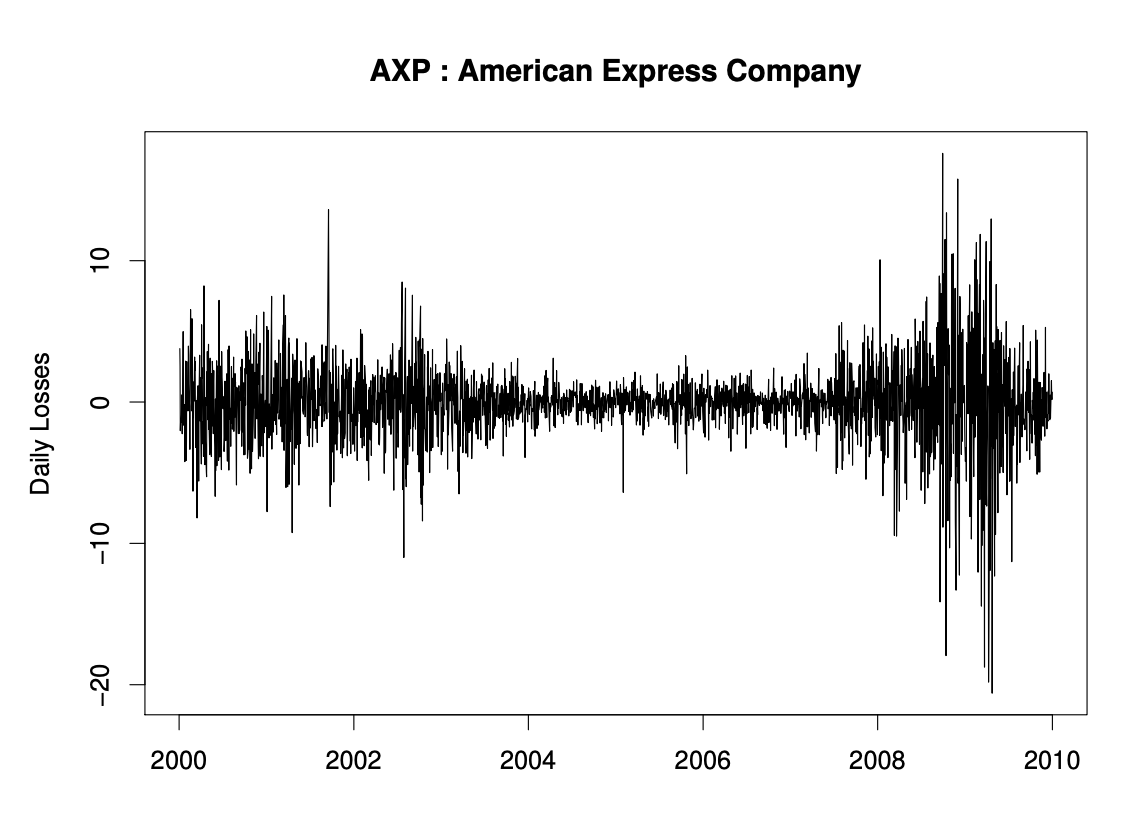
\includegraphics[width=2in]{notes/volatility.png}}
\end{center}
\end{figure}
We might be interested estimation of the VaR and ES conditional on the level of volatility. Here, volatility at time $t$ can be thought of as the potential energy carried in the graph up to time $t$. To condition of volatility, we must first specify a model for volatility dynamics. Let $\f_{t-1}$ denote the information set available at time $t-1$. To model timme-varying volatility, we fit multiplicative models to the process
\[r_t-\E(r_t|\f_{t-1})\]

\subsubsection{ARMA-GARCH Model}
The first model we use to model volatility is an $\text{ARMMA}(s,v)-\text{GARCH}(p,q)$ model defined as 
\begin{align*}
    r_t&= \kappa+ \sum_{h=1}^s\phi_hr_{t-h} + \sum_{l=1}^v \vartheta_j\varepsilon_{t-l}+\varepsilon_t\\
    \varepsilon_t&= \sigma_tz_t\\
    \sigma_t^2&=\alpha_0 + \sum_{i=1}^p\lambda_i\varepsilon_{t-i}^2+\sum_{j=1}^q\gamma_j\sigma_{t-j}^2
\end{align*}
Where $z_t$ are iid innovations with some unknown distribution function $G$, with $\E(z_t)=0$ and Var($z_t$)=1. We assume that the ARMA parameters $(\kappa, \phi_h)$ and the GARCH parameters $(\alpha_0>0, \lambda_i,\gamma_i\geq 0)$ all satisfy the necessary constraints for stationarity. Additionally, any fixed $t$, $\sigma_t$ and $z_t$ are independent.

\noindent After we fit this model to retrieve the all parameter estimates, we will perform extreme value analysis on the fitted scaled residuals of the volatility dynamics model $\hat{z}_t= \frac{\hat{\varepsilon}_t}{\hat{\sigma}_t}$. For this reason, it is crucial that our estimators from the volatility dynamics modeling have good properties. When the innovations have a finite moment (i.e. $\E(z_t^4)<\infty$), the quasi-maximum likelihood estimators of ARCH-GARCH models are consistent and asymptotically normal. In practice, $\E(z_t^4)$ is not finite for many series. Not only is this an issue but there is domain knowledge that is not take into consideration.
\subsubsection{AR-GJR-GARCH Model}
 Economic theory suggests that market information should have an asymmetric influence on volatility and empirical analyses show that positive and negative impact on conditional volatility. This gives rise to a GARCH model that applies \textbf{leverage}. The leverage effect is caused by the fact that negative returns have a higher influence on future volatility than positive returns. In order to incorporate leverage into a GARCH model, we fit an AR($p$)-GJR-GARCH(1,1) model to financial losses $r_t$. 
 \begin{align*}
     r_t&= \phi_0+\sum_{h=1}^p\phi_hr_{t-h}+ \varepsilon_t\\
     \varepsilon_t&= \sigma_tz_t\\
     \sigma_t^2&= \alpha_0+\lambda(|\varepsilon_{t-1}|-\gamma\varepsilon_{t-1})^2+\kappa\sigma_{t-1}^2
 \end{align*}
 where $(\phi_0,\hdots,\phi_p)$ lies in a compact subset of $\mathbb{R}^{p-1}$, $\alpha_0>0, \lambda\geq 0, 0\geq \kappa <1,$ and $-1\leq \gamma\leq 1$. As before, for any fixed $t$, $\sigma_t$ and $z_t$ are independent and $z_t$ are iid innovations with an unknown distribution function $G$. With the parameter vectore defined as bellow
\[\theta=(\phi_0, \hdots, \phi_p, \alpha_0, \lambda, \gamma, \kappa)\]
It has been shown that the global Gaussian quasi maximum likelihood estimator (QMLE) is strongly consistent (meaning that $\hat\theta_T \rightarrow \theta_0$ almost surely if the following conditions hold:
\begin{enumerate}
    \item The random variable $z_t$ are stationary and ergodic
    \item $\E[\ln(\kappa+\lambda(|z_t|-\gamma z_t)^2]<0$
    \item $\E[|z_t|^{2r}]<\infty$ and $\E[(\kappa+\lambda(|z_t|-\gamma z_t)^2)^r|\f_{t-1}^z]\leq C <1$ almost surely for some $r>0$
    \item $1-\sum_{j=1}^p \phi_jx^k\neq0, |x|\leq 1$
    \item $\E[z_t|\f_{t-1}^z]=0$ and  $\E[z_t^2|\f_{t-1}^z]=1$ almost surely
    \item for all $t$, the conditional distribution of $z_t$ given $\f^z_{t-1}$ is not
concentrated at two points
    \item $\kappa>0$
\end{enumerate}
This means that the QMLE is consistent (even for heavy tailed innovation distributions) as long as they have a finite moment. If our model is correctly specified, the the scaled residuals
\[\hat{z}_t=\frac{\hat\varepsilon_t}{\hat\sigma_t}\]
Should resemble an iid sequence from the generating distribution function $G$. These scale residuals are used to check the adequacy of the dynamic model and used as input for the extreme value analysis stage of our method. 
\subsection{Modeling the Innovation Distribution}
Although GARCH processes are known to be Pareto-like and heavy tailed, the scaled residuals may have (significantly) thinner tails than the original series. As we are interested in the conditional return distribution, our interests lie in the tail index of the innovations distribution. For a series that is AR($p$)-GARCH(1,1), there is no result to estimate the tail thickness. In fact, scaled residuals of these models tend to cluster above high levels. This means the scaled residuals still have dependence in extreme values. We could decluster these scaled residuals and then fit a GPD to threshold exceedences, but this approach is less than optimal. As these will result in difficulties when getting estimates for VaR and ES. The ideal approach would consist of eliminating all non-stationarity at all levels (including innovation distribution) and then use a large enough threshold in GP analysis such that clustering is not an issue. 

\subsection{Estimation Details}
The actual fitting process is as follows. Consider using data for day $t=1,\hdots, T$ to perform analysis.
\begin{enumerate}
    \item We fit an AR($p$)-GJR-GARCH(1,1) model using $p=3$. This is use because we do not know the distribution of the QMLE under the standard AR($p$)-GJR-GARCH(1,1) model. Our hope is that setting $p=3$ gives us a sufficiently flexible model that contains the true model.
    \item We calculate the scaled residuals
    \[\hat{z}_t= \frac{\hat\varepsilon_t}{\hat\sigma_t}\]
    After which we need to check our residuals. To do so, we use the Ljung-Box portmanteau test on the residuals and the squared residuals. If we get a large enough p value, we cannot reject the null hypothesis of no autocorrelation and assume that our model is successfully modeling the serial correlation structure in the conditional mean and the conditional variance of our data. After this, we use the intervals estimator of Ferro and Segers (discussed in section 5.2.5) to estimate the extremal index.
    \item Given no evidence of clustering (the extremal index is close to 1), we fit a $GP(\beta,\xi)$ to the points
    \[(z_{(n-k+1)}- z_{n-1}), \hdots, (z_{(n)}- z_{(n-k)}) \]
    where $z_{(n-k)}$ is the order statistic used as a threshold.
    \item The tail estimator for $F_Z(z)$ then takes the form
    \[\widehat{F_Z(z)}= 1- \frac{1}{k} \bigg( 1 +\hat\xi \frac{z-z_{(n-k)}}{\hat\beta} \bigg)^{-1/\hat\xi}\]
    \item For $q>1-\frac{k}{n}$, we can invert the tail formula and get a form for the $q^{th}$ upper quantile of the marginal distribution of $Z_t$
    \[\hat{z}_q= z_{(n-k)}+\frac{\hat\beta}{\hat\xi} \bigg( \big(\frac{1-q}{k/n}  \big)^{-\hat\xi}-1 \bigg)\]
\end{enumerate}
\subsubsection{Computing VaR and ES}
To compute the VaR and ES, we need the one-step ahead predictions for the conditional mean and the volatility. To calculate these, we use our estimates in the usual AR(3)-GJR-GARCH(1,1) equation:
\begin{align*}
    \hat{r}_{T+1}&= \hat{\phi}_0+\sum_{h=1}^3\hat{\phi}_hr_{T-h+1}\\
    \hat\sigma_{T+1}&= (\hat{\alpha_0}+\hat\lambda (|\hat\varepsilon_T|-\hat\gamma\hat\varepsilon_T)^2 +\hat\kappa\hat\sigma_T^2)^{\frac{1}{2}}
\end{align*}
Once we have these, we compute our statistics:
\begin{align*}
    \widehat{\text{VaR}}_T(q)&= \hat{r}_{T+1}+ \hat{z}_q\hat\sigma_{T+1}\\
    \widehat{\text{ES}}_T(q)&= \hat{r}_{T+1}+ \hat{z}_q\hat\sigma_{T+1} \bigg( \frac{1}{1-\hat\xi} +\frac{\hat\beta - \hat\xi z_{(n-k)}}{(1-\hat\xi)\hat{z}_q} \bigg)
\end{align*}
\subsection{Back Testing}
To assess the performance of the extreme value approach, we perform back testing on VaR and ES estimates. We use a backward window of 1000 days to estimate the model each time. For example, we can analyze the distribution of the $\xi$ parameter over the back test period. Through this, we can assess the consistency of $\theta$ \footnote{TODO MAKE BETTER}. We can also use back testing to compare our data observations to VaR and ES. 
\subsubsection{Back Testing VaR}
We record the number of cases where the return losses were greater than the VaR estimate. Using 
\[P(t_{t+1}>\text{VaR}_t(q))= 1-q\]
we know the probability of a violation is $1-q$. Let $C$ be the number of points we are back testing. We then use it to carry out the binomial test. The expected number of violations is the probability of a violation times the number of points we are back testing
\[T=C(1-q)\]
Under the null hypothesis, the model correctly identifies conditional quantiles and the expected number of violations follows a binomial distribution: $T\sim \text{Binom}(C, 1-q)$. We then perform a two sided binomial test of the null hypothesis against the alternative hypothesis that the estimates have systematic estimation error and give too few or too many violations.
\subsubsection{Back Testing ES}
The ES is the preferred measure of market risk as it gives some information about the size of potential losses given that a loss bigger that VaR has occurred. Under the null hypothesis that we correctly estimate the dynamics of the model and the first moment of the truncated innovation distribution ($\E[Z|Z>\text{VaR}_t(0.99)]$) the quantity below should behave like an iid sample with mean 0.
\[\hat\sigma_{t+1}^{-1}(r_{t+1} - \widehat{\text{ES}}_t(0.99))\]
We test this mean zero hypothesis using a bootstrap test.
\subsubsection{Batch Testing Extremal index}
When back testing, it is important that the estimated value of the extremal index following the intervals estimator is equal to 1.
\subsection{Discussion}
When using the two stage approach, the error from the time series modeling propagates through to the distributional fitting of the innovations in the second stage. This results in difficulties when quantifying the overall error. However, it has been shown that a two stage approach still provides good conditional VaR and ES forecast under mis-specification (Jalal and Rockinger (2008)).

\subsection{Realizing the Extremes}
While using an AR($p$)-GJR-GARCH(1,1) model works well for pre-whitening the data, it is often better to use a high frequency based volatility model. These are called realized EVT models. While the GARCH models filter the dependence adequately the realized EVT models perform better at forecasting especially at longer time horizons. 
\subsubsection{Theory of Realized Measures}
Let $p_t$ be the logarithmic price at time $t$ and define the conditional log-returns as
\begin{align*}
    p_t-p_{t-1}&=r_t=\mu_t+\sigma_t\varepsilon_t\\
    y_y&=f(\f_{t-1})\\
    \sigma_t^2&=h(\mathcal{H}_{t-1})
\end{align*}
where $\varepsilon_t$ is an iid process with zero mean and unit variance, $\mu_t$ is the conditional mean, and $\sigma_t^2$ is the conditional variance. These moments are functions of the information sets $\f_{t-1}$ and $\mathcal{H}_{t-1}$. The idea is to incorporate high frequency (intra daily) information in these sets. Assuming $\mu_t$ is constant, we specify a class of high-frequency based volatility models for the variable $\sigma_t^2$ using as a proxy the realized volatility $(RV)$. Here, $RV$ serves as a non-parametric estimator of the variation of the price path of an asset obtained by the sum of square of intra-day returns. Let 
\[r_{t,\Delta}= p_t-p_{t-\Delta}\]
With $t_{t,\delta}$ denoting the discretely sampled $\Delta-$period return, we define $RV$ on day $t$ as 
\[RV_t= \sum_{j=1}^Nr^2_{t-1+(j\cdot \Delta),\Delta}\]
We assume the $\sigma_t^2$ is defined as a function of the conditional $RV$ as below
\[\sigma_t^2=g(\E[RV_t|\mathcal{H}_{t-1}])\]
\subsubsection{Modeling Realized Extremes}
To model volatility (given by $\sigma_t^2$), we must specify a model for the conditional expectation of the $RV$ and a ling function $g$ that maps the conditional mean of the $RV$ to the conditional variance of the returns. For this purpose, we use the heterogeneous autoregressive (HAR) class of models. Let the multi-period normalized $RV$ be denoted by
\[RV_{t,t+h}=\frac{1}{h}[RV_{t+1}+ \hdots+RV_{t+h}]\]
The daily HAR model can be expressed as 
\[\log(RV_{t,t+h}) = \beta_0+ \beta_D\log(RV_t)+\beta_W\log(RV_{t-5,t})+\beta_M\log(RV_{t-22,t})+\eta_{t,t+h}\]
We see that this specification exploits the information from the 1-day $RV$, the 5-day average $RV$ and the 22-day average $RV$ thus reflecting the idea that heterogeneity in investor behavior creates different volatility components having different impacts on the future volatility. Now that we have a model for the conditional expectation of the $RV$, we can focus on specifying our link function $g$. The following are the 3 most likely choices:

\begin{align*}
    \hat\sigma_{t,t+h}^2&=  \exp\bigg( \widehat{\log(RV_{t,t+h})} \bigg)\\
    \hat\sigma_{t,t+h}^2&=  c+ d\exp\bigg( \widehat{\log(RV_{t,t+h})} \bigg)\\
    \hat\sigma_{t,t+h}^2&= c + d \exp\bigg( \widehat{\log(RV_{t,t+h})} +0.5\hat\sigma_{\hat\eta}^2 \bigg)
\end{align*}
Where $c,d$ are coefficients to be estimated and $\hat\sigma_{\hat\eta}^2$ is the estimated variance of the logarithmic HAR regression residuals.
\subsubsection{Summary of Realized EVT Approach}
The realized EVT approach the amounts to
\begin{enumerate}
    \item Fitting a high frequency based model for conditional variance
    \item Filtering the returns (effectiveness measured with extremal index)
    \item Fitting a GP model on the tails to obtain a tail estimator
    \item $h$-day ahead prediction of VaR and ES using the tail estimator for the residuals and $h$-period forecasts of the conditional mean and variance obtained from fitting HAR model directly onto the multi-period $RV$.
\end{enumerate}



\end{document}